\newpage
\section{Example 2: Identification of speech in noise using an adaptive method}

\subsection{General description of the experiment}
See \filename{examples/manual/sentenceinnoise.apx}. This is an
example of an adaptive speech in noise test. It determines the
 \ac{srt}, the 50 percent correct point, using
the 1-down, 1-up method described by \citet{PM79}. In this
adaptive procedure the first sentence is repeated with increasing
level until it is identified correctly. Subsequently, the SRT is
determined by increasing or decreasing the level in steps of 2 dB,
according to the last response. Other decision procedures (eg
2-down 1-up) can also be implemented using \apex. In this example
the 5 sentences are scored on the basis of their keywords. The
keywords are indicated in bold on the screen. The
experimenter/clinician is seated in front of the screen and
decides whether the subject has repeated the keywords (of the
sentence) correctly, after which the correct or incorrect button
is clicked(figure~\ref{fig:sentencenoise}). No feedback is
provided. The starting level is given in signal-to noise ratio
(the level of the noise remains the same, that of the signal
varies). In this example speech and noise are routed to the same
channel, i.e. one speaker or one earpiece of the headphone. The
results are written to a results file.

\begin{figure}
 \centering
 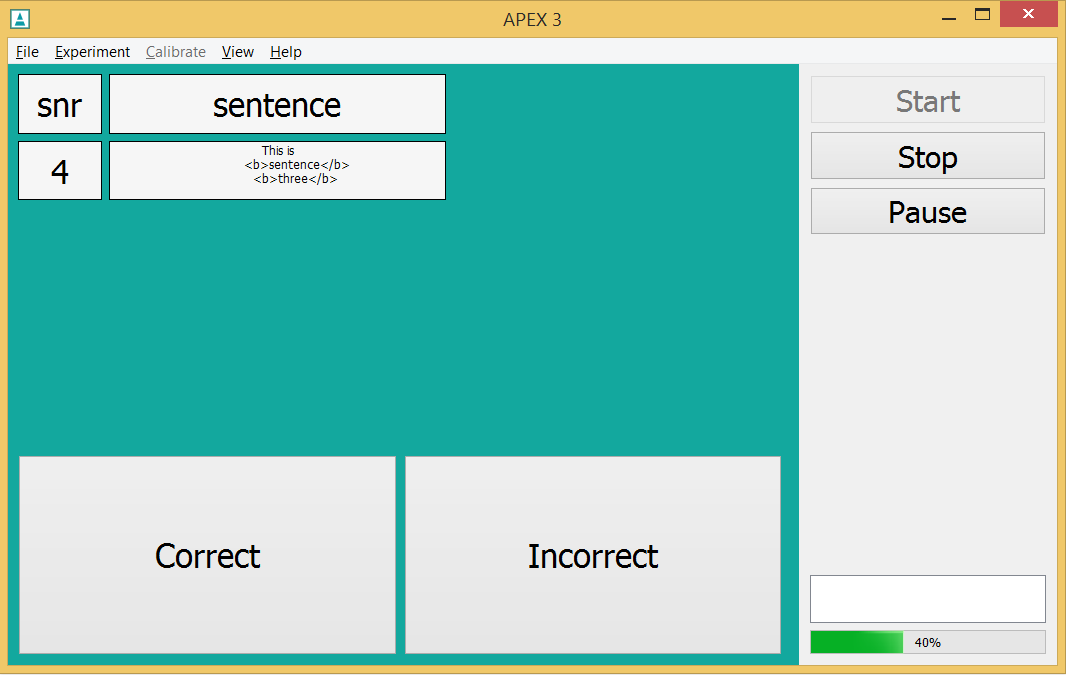
\includegraphics[width=\textwidth]{example2sentenceinnoise.png}
 \caption{Example of adaptive sentence in noise experiment}
 \label{fig:sentencenoise} \todo{bold werkt niet correct?}

\end{figure}
\subsection{Conceptual}
The experiment as described in the previous paragraph should first
be translated to concepts understood by \apex. The main concepts
in this example are \textbf{datablock}, \textbf{stimulus},
\textbf{screen}, \textbf{procedure}, a \textbf{variable} parameter
(to change the gain) and \textbf{fixed Parameter} to show a
sentence on the screen. For each sentence a datablock is defined,
and for each resulting datablock a stimulus is defined. As always,
everything that is defined, is assigned an ID, to be able to refer
to it later on. In this example there are 5 stimuli with IDs
\id{stimulus_sentence1}, \id{stimulus_sentence2},
\id{stimulus_sentence3}, \id{stimulus_sentence4} and
\id{stimulus_sentence5}. The procedure defines a number of trials.
Recall that a trial is the combination of a screen (always the
same in this example), a stimulus and a response.

As we are dealing with an adaptive procedure a fixed or variable
parameter is adapted. In this example a variable parameter is
adapted to change the gain of the sentence, and a fixed parameter
is used to show a sentence on the screen. The screen also shows
the signal-to-noise ratio (SNR) under test and the response
alternatives ``correct'' and ``incorrect''.

Now only the output logic remains to be defined. The idea is to
continuously present a noise signal and to vary the level of the
sentences adaptively. To achieve this, we define 2 filters, the
first one is a generator (i.e., a filter without input channels)
that will generate the noise signal. The other one is an
amplifier, which will amplify or attenuate the sentences to obtain
the desired SNR. Both are connected to one channel of the
wavdevice.

In the following sections each of the elements of the XML file
necessary to implement the latter concepts will be described in
detail.

\subsection{Detailed description of various elements}

\begin{lstlisting}
<procedure xsi:type="apex:adaptiveProcedure">
  <parameters>
    <presentations>1</presentations>
    <order>sequential</order>
    <corrector xsi:type="apex:isequal"/>
    <nUp>1</nUp>
    <nDown>1</nDown>
    <adapt_parameter>gain</adapt_parameter>
    <start_value>0</start_value>
    <stop_after_type>presentations</stop_after_type>
    <stop_after>1</stop_after>
    <larger_is_easier>true</larger_is_easier>
    <repeat_first_until_correct>true</repeat_first_until_correct>
    <stepsizes><stepsize begin="0" size="2"/></stepsizes>
  </parameters>

  <trials>
    <trial id="trial_sentence1">
         <answer>button_correct</answer>
         <screen id="screen"/>
         <stimulus id="stimulus_sentence1"/>
    </trial>

    <trial id="trial_sentence2">
         <answer>button_correct</answer>
         <screen id="screen"/>
         <stimulus id="stimulus_sentence2"/>
    </trial>

    <trial id="trial_sentence3">
        <answer>button_correct</answer>
        <screen id="screen"/>
        <stimulus id="stimulus_sentence3"/>
    </trial>

    <trial id="trial_sentence4">
        <answer>button_correct</answer>
        <screen id="screen"/>
        <stimulus id="stimulus_sentence4"/>
    </trial>

    <trial id="trial_sentence5">
        <answer>button_correct</answer>
        <screen id="screen"/>
        <stimulus id="stimulus_sentence5"/>
    </trial>
  </trials>
</procedure>
\end{lstlisting}


The attribute \xml{xsi:type="adaptiveProcedureType"} of
\element{procedure} refers to a procedure in which a parameter is
changed according to the response of the subject. In this example
the gain of the amplifier is adapted. The procedure selects the
next trial from the trial list and it completes after every trial
has been presented a certain number of times.

\begin{itemize}
\item \element{parameters} defines the behavior of the procedure

\begin{itemize}

\item \element{presentations} every trial is presented once

\item \element{order} the trials are presented sequentially, in
the order that is specified in the experiment file (if
\xml{random} would be specified, they would be presented in random
order).

\item \element{corrector} the corrector checks whether the response is correct or not. The
attribute \xml{xsi:type="apex:isequal"} compares whether the two
input values are exactly the same. In this example
\element{corrector} compares the answer specified under trial  (\id{button_correct}) and
the ID corresponding to the picture that has been clicked (either \id{button_correct} or \id{button_incorrect}).

\item \element{nUp} the level is increased after n (here 1)
incorrect response(s); cf \element{larger_is_easier}

\item \element{nDown} the level is decreased after n (here 1)
correct response(s); cf \element{larger_is_easier}

\item \element{adapt_parameter} to be adapted

\item \element{start_value} the experiment starts with gain=0
(input of user). The value here will be replaced by the entry
value. Please refer to section~\ref{sec:Interactive} for more
information.

\item \element{stop_after_type} the experiment stops after a
specified number of presentations of each trial is completed (it
is also possible to stop after \element{reversals}.

\item \element{stop_after} the experiment stops after 1
presentation of each trial

\item \element{larger_is_easier} If \xml{true}, then larger values
of the parameter are easier than smaller values. It is used to
determine \element{nUp} and \element{nDown}.

\item \element{repeat_first_until_correct} the first trial is
repeated with increasing gain until it is identified correctly.

\item \element{stepsizes} from the beginning of the experiment
(begin=0) the stepsize is 2 dB.
\end{itemize}

\item \element{trials} contains different \element{trial} elements
to specify a trial. Once a trial is selected, \element{procedure}
will show the specified screen and send the stimulus to the
device. Each trial is given an ID (arbitrary name), eg
\id{trialsentence1}, such that it can be referred to later on or
viewed in the results file. A trial must be defined for all the
sentences of the experiment.

\item \element{answer} the correct answer, to be used by \apex to
determine whether the subject's response is correct. In this
example the experimenter will click on ``correct'' or
``incorrect''. The result from the screen will be the ID of the
element of the screen that was clicked (\id{button_correct} or
\id{button_incorrect}).

\end{itemize}

\index{parameters}

\index{procedure}

\index{presentations}

\index{order}

\index{corrector}

\index{nUp}

\index{nDown}

\index{adapt parameter}

\index{start value}

\index{stop after type}

\index{stop after}

\index{larger is easier}

\index{repeat first until}

\index{stepsizes}

\index{trial}

\index{answer}

\begin{lstlisting}
<screens>
        <reinforcement>
            <progressbar>true</progressbar>
            <feedback length="600">false</feedback>
        </reinforcement>

        <screen id="screen">
       <gridLayout height="2" width="1" id="main_layout" rowstretch="1,2">
               <gridLayout width="4" height="4" columnstretch="1,4,2,2"
               rowstretch="1,1,2,2" id="parameter_layout" row="1" col="1">

    <label id="snrlabel" row="1" col="1">
    <text>snr</text>
    </label>

    <parameterlabel id="snr" row="2" col="1">
      <parameter>gain</parameter>
    </parameterlabel>

    <label id="sentence" row="1" col="2">
    <text>sentence</text>
    </label>

    <parameterlabel id="sentence" row="2" col="2">
    <fontsize>12</fontsize>
    <parameter>sentence</parameter>
    </parameterlabel>

    </gridLayout>

    <gridLayout height="1" width="2" id="answer_layout" x="1" y="2">
    <button x="1" y="1" id="button_correct">
    <text>Correct</text>
     </button>
    <button x="2" y="1" id="button_wrong">
    <text>Incorrect</text>
    </button>

    </gridLayout>
    </gridLayout>
    <buttongroup id="buttongroup">
    <button id="button_correct"/>
    <button id="button_wrong"/>
    </buttongroup>
    <default_answer_element>buttongroup</default_answer_element>
    </screen>
    </screens>>
\end{lstlisting}

\element{screens} contains \element{screen} element that is
referred to in \element{procedure}.

\begin{itemize}
\item \element{reinforcement} includes elements on progress and
feedback
\begin{itemize}

\item \element{progressbar} If the value is \xml {true} a progress
bar will be displayed in the right hand bottom corner of the
screen that indicates the percentage of trials that have been completed.

\item \element{feedback length} duration of the time after
response (in msec) that \apex waits before presenting the next
trial. During this interval feedback can be displayed. In this
example, no feedback (thumb up, thumb down) is given as the value
is \xml{false}.
\end{itemize}

\item \element{screen} the screen has an ID by which it can be
referred to in each trial. In this example the screen displays
four blocks in the top left corner to indicate the SNR and the
sentence. In addition, the labels ``Correct'' and ``Incorrect''
are displayed on the buttons at the bottom of the screen (cfr
screenshot, figure...).
\begin{itemize}

\item \element{gridlayout} places elements in an irregular grid.
The screen is divided into sections according to the values. In
this example there are two nested layouts. The main layout divides the screen in two main rows (height = 2, width = 1).
The parameter layout divides the first of these rows in four rows and four columns, of which only the two first ones are filled.
The answer layout divides the second main row in two columns, each with one button.
The stretch factor for the columns is a list of integers, separated by
comma's. There should be as many integers as columns. The width of
the columns is proportional to the numbers. With \xml{width="1"},
and \xml{height="2"} \xml{rowstretch="1,2"} implies that the
second row will be twice as wide as the first one. If
\xml{width="4"}, and \xml{height="4"} and
\xml{columnstretch="1,4,2,2"} the second column will be four times
as wide as the first and two times as wide as the 3rd and 4th.
With \xml{columnstretch="1,1,2,2"} the 3rd and 4th rows will be
twice as wide as the 1st and 2nd.

\item \element{label} the labels on the left are fixed and display
the \element{text} ``SNR'' and ``Sentence''. The button
``Correct'' and ``Incorrect'' are indicated at the bottom of the
screen

\item \element{parameterlabel} the blocks on the right display the values
of the fixed parameters. Gain is the (variable) SNR level, and
sentence is a fixed parameter, defined in \element{stimulus}

\item \element{font size} can be specified in points

\item \element{buttongroup} defines a group of screen elements
(those that are displayed on the screen). As many elements can be
defined in a screen, \apex has no way to know which element
contains the subject's response. Therefore, in
\element{default_answer_element} the element is designated that
contains the subject's response. In the case of screen elements
that are clicked in order to respond, the example is further
complicated by the fact that we cannot specify just one of the
elements (one button, one picture), but that the response rather comes
from a group of elements. This is when a \element{buttongroup} can
be used to group together different screen elements.


\end{itemize}
\end{itemize}
\index{screens} \index{reinforcement} \index{progressbar}
\index{feedback} \index{screen} \index{gridlayout} \index{label}
\index{parameter label} \index{font size} \index{buttongroup}
\index{default answer element}

\begin{lstlisting}
<datablocks>
  <uri_prefix>sentences/</uri_prefix>
  <datablock id="datablock_sentence1">
    <device>wavdevice</device>
    <uri>sent1.wav</uri>
  </datablock>
  <datablock id="datablock_sentence2">
    <device>wavdevice</device>
    <uri>sent2.wav</uri>
  </datablock>
  <datablock id="datablock_sentence3">
    <device>wavdevice</device>
    <uri>sent3.wav</uri>
  </datablock>
  <datablock id="datablock_sentence4">
    <device>wavdevice</device>
    <uri>sent4.wav</uri>
  </datablock>
  <datablock id="datablock_sentence5">
    <device>wavdevice</device>
    <uri>sent5.wav</uri>
  </datablock>
  <datablock id="noisedata">
    <device>wavdevice</device>
    <uri>noise.wav</uri>
  </datablock>
  <datablock id="silence">
    <device>wavdevice</device>
    <uri>silence:500</uri>
  </datablock>
</datablocks>
\end{lstlisting}


\element{datablocks} contains a list of \element{datablock}
elements and a prefix.
\begin{itemize}
\item \element{uri_prefix} a relative path is specified here
(relative with respect to the experiment file). Since \apex knows
the location of the experiment file, only the folder containing
the wave files and pictures must be specified. It is also possible
to give the absolute path, starting at the root. There are 3 ways
to specify a prefix: by directly specifying an absolute path, by
directly specifying a path relative to the experiment file or by
referring to a prefix stored in \filename{apexconfig.xml}. Please
refer to section~\ref{sec:prefixes} for more information. \todo{necessary to repeat all this information here, not enough to refer to prefixes section? (Lot)}

\item \element{datablock} for each wave file a datablock is made,
with an ID.

In datablock \id{silence} the special syntax is
demonstrated for creating a datablock containing only silence
(i.e., zeros). This is done to put silence before and after the
sentence, to prevent the speech and noise from
starting at the same time. The length of the silence datablock is
specified in ms after the prefix \xml{silence}. It is added before the signal (in element \element{stimulus}), not
before the noise.

\begin{itemize}
\item the datablock is associated with the sound card with ID
\id{wavdevice}, as defined in the \element{devices} section.

\item \element{uri} the URI is appended to the prefix defined
above

\end{itemize}
\end{itemize}
\index{uri prefix}

\index{datablocks}

\index{datablock}

\index{device}

\index{uri}


\begin{lstlisting}
<devices>
    <device id="wavdevice" xsi:type="apex:wavDeviceType">
    <driver>portaudio</driver>
    <card>default</card>
    <channels>1</channels>
    <samplerate>44100</samplerate>
    </device>
</devices>
\end{lstlisting}

All devices defined in the experiment file are grouped in
\element{devices}.The ID is set to \id{wavdevice}. As an ID is
unique for an entire experiment file, it can be used later on to
refer to this device (eg in datablocks).

\begin{itemize}
\item \element{device} the \xml{xsi:type="apex:wavDeviceType"}
attribute tells \apex that a sound card is used. The experiment
only starts if all devices can be opened.

\item \element{driver} specifies the software driver to be used
for sound output. If unsure, set it to \xml{portaudio}.

\item \element{card} specifies the name of the sound card to be
used. The system default card can be used by specifying
\xml{default} as a card name. Other card names can be defined in
\filename{apexconfig.xml}.

\item \element{samplerate} the sampling frequency of the sound
card. Not all sampling rates are supported by all devices, and
some drivers automatically convert the sampling rate. Check your
sound card documentation. The sample rate of the sound card should
correspond to the sampling rates of all \element{datablocks} used
with it.
\end{itemize}

\index{device} \index{driver} \index{card} \index{channels}
\index{gain} \index{samplerate}

\begin{lstlisting}
<filters>
<filter xsi:type="apex:dataloop" id="noisegen">
    <device>wavdevice</device>
    <channels>1</channels>
    <continuous>false</continuous>
    <datablock>noisedata</datablock>
    <basegain>-5</basegain>
    <gain>0</gain>
    <randomjump>true</randomjump>
    </filter>
<filter xsi:type="apex:amplifier" id="amplifier" >
    <device>wavdevice</device>
    <channels>1</channels>
    <basegain>-5</basegain>
    <gain id="gain">0</gain>
</filter>
</filters>
\end{lstlisting}

\element{filters} contains individual \element{filter} elements,
which specify a filter, or as a special case a generator (i.e., a
filter without input channels).

\begin{itemize}

\item The attribute \xml{xsi:type="apex:dataloop"} tells \apex
that a dataloop generator has to be created. This is a generator
that takes a datablock and loops it infinitely. The datablock to
be looped is specified by its ID \id {noisedata}.

\item \element{filter} on line~\ref{xml:filter2} the attribute
\xml{xsi:type="apex:amplifier"} tells \apex that an amplifier has
to be created. The gain of this amplifier will be varied to change
the amplitude of the words and thus the SNR. It is assigned ID
\id{amplifier}. The gain of the amplifier is made a variable
parameter by assigning it ID \id{gain}

\begin{itemize}

\item \element{device} the device with which the filter is
associated

\item \element{channels} The number of channels of the filter. The
available number of channels depends on the type of filter. An
amplifier can have any number of channels.

\item \element{continuous} If set to \xml{false} the noise is
presented during the speech, but not during the subject's
response.

\item \element{datablock} the datablock with ID noisedata,
specified under \element{datablocks} will be looped.

\item \element{basegain}:  the total gain of the amplifier is
basegain+gain. The total gain of the complete output system should
not be larger than 0 to avoid clipping of the signal. This is why
basegain = -5.

\item \element{gain} the gain value that is changed. E.g. if the
targetamplitude is 65 dB SPL (see Calibration) the signal and
noise have equal amplitude if gain = 0. Gain is changed by other
modules.

\item If \element{randomjump} is set to \xml{true}, when the
dataloop is started, it will jump to a random sample in the
datablock. Thereafter it is looped.

\end{itemize}

\end{itemize}
\index{filters} \index{filter} \index{device} \index{channels}
\index{continuous} \index{datablock} \index{basegain} \index{gain}
\index{randomjump}

\begin{lstlisting}
<stimuli>
  <fixed_parameters>
    <parameter id="sentence"/>
  </fixed_parameters>

  <stimulus id="stimulus_sentence1">
    <datablocks>
    <sequential>
        <datablock id="silence"/>
        <datablock id="datablock_sentence1"/>
        <datablock id="silence"/>
    </sequential>
    </datablocks>

  <fixedParameters>
    <parameter id="sentence">This is <b> sentence </b> <b>one</b></parameter>
  </fixedParameters>
  </stimulus>

  <stimulus id="stimulus_sentence2">
    <datablocks>
    <sequential>
        <datablock id="silence"/>
        <datablock id="datablock_sentence2"/>
        <datablock id="silence"/>
    </sequential>
    </datablocks>

  <fixedParameters>
    <parameter id="sentence">This is <b> sentence </b> <b>two</b></parameter>
    </fixedParameters> </stimulus>

  <stimulus id="stimulus_sentence3">
    <datablocks>
    <sequential>
        <datablock id="silence"/>
        <datablock id="datablock_sentence3"/>
        <datablock id="silence"/>
    </sequential>
    </datablocks>

<fixedParameters>
<parameter id="sentence">This is <b> sentence </b> <b>three</b></parameter>
</fixedParameters>
</stimulus>

<stimulus id="stimulus_sentence4">
    <datablocks>
    <sequential>
        <datablock id="silence"/>
        <datablock id="datablock_sentence4"/>
        <datablock id="silence"/>
    </sequential>
    </datablocks>

<fixedParameters>
<parameter id="sentence">This is <b> sentence </b> <b>four</b></parameter>
</fixedParameters>
</stimulus>

<stimulus id="stimulus_sentence5">
    <datablocks>
    <sequential>
        <datablock id="silence"/>
        <datablock id="datablock_sentence5"/>
        <datablock id="silence"/>
    </sequential>
    </datablocks>

   <fixedParameters> <parameter id="sentence">This is <b> sentence
   </b> <b>five</b> </parameter> </fixedParameters> </stimulus>
</stimuli>
\end{lstlisting}

\element{stimuli} contains different \element{stimulus}, each with
an ID.

\begin{itemize}
\item \element{fixedParameters} is used here to be able to show
the sentence under test on the Screen. Fixed parameters are
discussed in section~\ref{sec:Parameters}.


\begin{itemize}
\item \element {parameter} the fixed parameter is defined here and
should also be defined in each \element {stimulus}
\end{itemize}

\item \element{stimulus} Each stimulus gets an ID (referred to in
\element {trial})
\begin{itemize}

\item \element{datablocks} here one refers to the
\element{datablock} described before; it includes the sentence
file.

\begin{itemize}
\item \element{sequential} The sequence of \element{datablocks} is
indicated here.
\end{itemize}

\item \element{fixedParameters} sets the fixed parameter for each
\element{stimulus}.

\item \element{b} indicates which words (the keywords) should
appear in bold on screen.
\end{itemize}
\end{itemize}

This is repeated for all the sentences.

\index{stimuli}

\index{fixed parameters}

\index{stimulus}

\index{datablocks}

\index{sequential}

\index{parameter}



\begin{lstlisting}
<connections>
    <connection>
        <from>
        <id>_ALL_</id>
        <channel>0</channel>
        </from>
        <to>
        <id>amplifier</id>
        <channel>0</channel>
        </to>
    </connection>
    <connection>                (*@\label{xml:ch1}@*)
        <from>
        <id>amplifier</id>
        <channel>0</channel>
        </from>
        <to>
        <id>wavdevice</id>
        <channel>0</channel>
        </to>
    </connection>               (*@\label{xml:ch2}@*)
    <connection>                (*@\label{xml:ch3}@*)
        <from>
        <id>noisegen</id>
        <channel>0</channel>
        </from>
        <to>
        <id>wavdevice</id>
        <channel>0</channel>
        </to>
        </connection>           (*@\label{xml:ch4}@*)
</connections>
\end{lstlisting}

\index{connections} \index{channel}

\begin{itemize}
\item \element{connections} defines how the different datablocks
and filters are routed to the output device. The ID \id{_ALL_}
stands for all the datablocks. In this example they are routed to
the first channel of the filter with ID {amplifier} (defined under
\element{filters}). In the amplifier the signal is amplified or
attenuated and sent to the wavdevice on lines~\ref{xml:ch1}
to~\ref{xml:ch2}. At the same time the noise, generated by a
generator with ID noisegen, is sent to the same channel of the
wavdevice. The channels are numbered from 0 onwards. The level of
the noise remains constant and does not pass through an amplifier
(lines~\ref{xml:ch3} to ~\ref{xml:ch4}). Although noisedata is a
\element{datablock} and connected to \emph{amplifier} it is not
specified in \element{stimulus} and does not pass through
\emph{amplifier}.
\end{itemize}

A visual representation of connections can be obtained by choosing
``Show stimulus connections'' under ``Experiment''in the main
\apex menu (top left menu bar).


\begin{lstlisting}
 <results>
  <page>apex:resultsviewer.html</page>
  <resultparameters>
   <parameter name="reversals for mean">4</parameter>
  </resultparameters>
  <showduringexperiment>false</showduringexperiment>
  <showafterexperiment>true</showafterexperiment>
  <saveprocessedresults>true</saveprocessedresults>
 </results>
\end{lstlisting}


\element{results} Even if \element{results} is not specified in
the experiment file \apex will save a results file in XML.

\todo{new part, to check!}
\begin{itemize} 
\item \element{page} URL of the html page to show in the results window. The page should have the appropriate java script methods embedded. More example pages can be found in the \apex resultsviewer folder.
\item \element{resultparameters} Parameters to be passed to the results page. Each parameter will be set in hash params. In this example, the result will be calculated as the mean of the variable parameter (gap) at the last 4 reversals.  \todo{what is hash params? (lot)}
\item \element{showduringexperiment} If true, an extra window will be created which will show the results of the current experiment while the experiment is being executed. Javascript embedded in the page will be executed upon each new trial.
\item \element{showafterexperiment} If true, when the experiment is finished, a dialog box will appear querying whether results should be shown. If the answer is affirmative, a new window will be opened and the results will be shown after javascript processing.
\item \element{saveprocessedresults} If \xml {true} the
experimenter will be asked whether the processed results must be
appended to the results file. This will only work if the results are successfully saved to disk and your javascript code supports this transformation.
\end{itemize}

\index{results} \index{page} \index{resultparameters} \index{showduringexperiment} \index{showafterexperiment} \index{saveprocessedresults}


\begin{lstlisting}
<interactive> <entry type="int" description="SNR start value"
  expression="/apex:apex/procedure/parameters/start_value" default="4" />
</interactive>
\end{lstlisting}

If a small part of an experiment file has to be changed right
before the start of an experiment (e.g. a start value, a gain
value, the subject's name), \apex can show the experimenter a
small \ac{gui} containing the elements to be changed. This is
accomplished by defining the \element{interactive} element in the
experiment file.

In this example we will modify the gain of the filter with ID
\id{amplifier} to a value that is entered by the experimenter at
the start of the experiment.

\begin{itemize}
\item \element{entry type} a value is entered, here corresponding
to SNR in dB. It is also possible to enter a string, e.g. name of
the subject (see Reference Manual).

\item \element{expression} the interactive window will show 4 as
default value; more than one entry may be defined.
\end{itemize}

\index{interactive}

\index{entry type}

\index{expression}
